\documentclass{article}

\usepackage[letterpaper, margin=1in]{geometry}
\usepackage{setspace}
\usepackage{amsmath,amssymb}
\usepackage{graphicx}
\usepackage[amsmath,thmmarks,framed]{ntheorem}
\usepackage[ruled,linesnumbered]{algorithm2e}
\usepackage{authblk}
\usepackage{tcolorbox}
\usepackage{xcolor}
\definecolor{darkgreen}{rgb}{0.0,0.5,0.0}
\usepackage[colorlinks,linkcolor=red,citecolor=darkgreen,urlcolor=blue]{hyperref}
\usepackage[round,authoryear]{natbib}

\newtheorem*{remark}{Remark}

\newcommand{\Le}{\leqslant}
\newcommand{\Ge}{\geqslant}
\newcommand{\D}{\mathrm{d}}
\newcommand{\DB}{\mathrm{DB}}
\newcommand{\KL}{\mathrm{KL}}
\newcommand{\TV}{\mathrm{TV}}
\newcommand{\Fish}{\mathrm{Fisher}}
\newcommand{\setzero}{\setlength{\itemsep}{0pt}}

\theoremstyle{plain}

\title{Detailed Balance Normalizing Flow for Multi-Modal Boltzmann Sampling}
\author[1]{Qi Feng}
\author[2]{Rongjie Lai}
\author[2]{Xuda Ye}
\affil[1]{Department of Mathematics, Florida State University, Tallahassee, FL 32306}
\affil[2]{Department of Mathematics, Purdue University, West Lafayette, IN 47907}

\date{\today}

\begin{document}
\maketitle

\section{Introduction}

Normalizing flows based on the KL divergence \citep{rezende2015variational} have been widely applied in generative sampling. In energy-based sampling from physical potentials, the Boltzmann generator \citep{noe2019boltzmann,wu2020stochastic} has been the industry standard for fast sampling from target Boltzmann distributions. Compared with classical Monte Carlo simulation, which suffers from slow convergence due to long mixing times and strong sample correlation, the Boltzmann generator overcomes this bottleneck and greatly accelerates inference by directly applying the trained flow map to push prior samples to the target, producing independent samples in a single forward pass.

Despite their popularity, KL normalizing flows suffer from several intrinsic drawbacks. First, the flow map is a diffeomorphism on the whole space, so for multi-modal distributions the resulting NF often introduces artificial bridges between modes. Second, the KL loss is highly sensitive to mode collapse, and the flow easily falls into a few dominant modes while neglecting the rest. Both drawbacks ultimately trace to the \emph{signed} nature of the KL integrand, which leaves no room to replace the inaccessible target by a more convenient surrogate without shifting the optimum.

In this paper, we propose a normalizing flow based on the detailed balance (DB) divergence, as an alternative to KL-based Boltzmann generators for energy-based sampling from multi-modal Boltzmann distributions. The DB divergence measures the score difference between two distributions in $L^1$, so its integrand is pointwise nonnegative; this single property allows the target $\mu_1$ in the forward loss to be replaced by an arbitrary positive guiding measure without disturbing the global minimizer, and is the basis for the mode-guidance mechanism that suppresses mode collapse. The construction incurs only a constant-factor overhead in training while offering substantially more flexibility in use.

The rest of the paper is organized as follows. Section~\ref{sec:db-divergence} introduces the DB divergence and places it among classical distribution metrics. Section~\ref{sec:single-step} builds the single-step DB normalizing flow, comprising a reverse DB loss for energy-based sampling, a forward DB loss for mode guiding, and a curvature-based construction of the guiding measure. Section~\ref{sec:db-bg} composes the single-step flow into a DB Boltzmann generator.

\section{Detailed balance divergence}\label{sec:db-divergence}

\subsection{Basic definition}

We introduce the detailed balance (DB) divergence to characterize the discrepancy between two distributions. The motivation is that score matching in $L^1$, rather than in $L^2$ as in the Fisher information, admits a direct PDE interpretation: the resulting Euler--Lagrange equation is the detailed balance condition itself, which links the divergence to the equilibrium structure of Langevin dynamics. Let $\mu$ and $\nu$ be probability distributions on $\mathbb R^d$. The DB divergence is defined as
\begin{equation}\label{eq:db-def}
    \DB(\nu\|\mu) = \int_{\mathbb R^d} \nu(x) \bigl|\nabla \log \nu(x) - \nabla \log \mu(x) \bigr| \D x = \int_{\mathbb R^d} \mu(x) \biggl|\nabla\biggl(\frac{\nu(x)}{\mu(x)}\biggr)\biggr| \D x,
\end{equation}
which is reminiscent of both the KL divergence
\begin{equation*}
    \KL(\nu\|\mu) = \int_{\mathbb R^d} \nu(x) \log \frac{\nu(x)}{\mu(x)} \D x,
\end{equation*}
and the Fisher information
\begin{equation*}
    \Fish(\nu\|\mu) = \int_{\mathbb R^d} \nu(x) \bigl|\nabla \log \nu(x) - \nabla \log \mu(x) \bigr|^2 \D x.
\end{equation*}
By definition, $\DB(\nu\|\mu)$ is nonsymmetric and nonnegative, and it vanishes precisely when the ratio $\nu(x)/\mu(x)$ is constant, that is, when $\mu = \nu$.

If $\mu$ takes the unnormalized form $\mu(x) \propto e^{-U(x)}$ with potential $U(x)$, then
\begin{equation*}
    \DB(\nu \| \mu) = \int_{\mathbb R^d} \bigl|\nabla \nu(x) + \nu(x)\nabla U(x) \bigr| \D x,
\end{equation*}
so minimizing the DB divergence amounts to solving the PDE
\begin{equation}\label{eq:db-pde}
    \nabla \nu(x) + \nu(x) \nabla U(x) = 0,
\end{equation}
which is exactly the detailed balance condition for sampling $e^{-U(x)}$ via Langevin dynamics. The DB divergence therefore carries a natural physical meaning.

\subsection{Relations to other distribution metrics}

The DB divergence is closely related to two classical distribution metrics, the Fisher information and the total variation distance, and sits naturally between the two in strength.

\paragraph{Fisher information.}
The Fisher information of $\nu$ relative to $\mu$ is
\begin{equation*}
    \Fish(\nu \| \mu) = \int_{\mathbb R^d} \nu(x) \bigl|\nabla \log \nu(x) - \nabla \log \mu(x) \bigr|^2 \D x,
\end{equation*}
so by~\eqref{eq:db-def} the DB divergence is precisely its $L^1$ counterpart, with the squared $L^2$ norm of the score difference replaced by an $L^1$ norm. The Cauchy--Schwarz inequality together with $\int \nu(x) \D x = 1$ then yields
\begin{equation}\label{eq:db-fisher}
    \DB(\nu \| \mu)^2 \Le \Fish(\nu \| \mu).
\end{equation}

\paragraph{Total variation distance.}
The total variation distance between $\mu$ and $\nu$ is
\begin{equation*}
    \TV(\mu, \nu) = \frac{1}{2} \int_{\mathbb R^d} |\mu(x) - \nu(x)| \D x.
\end{equation*}
Setting $f(x) = \nu(x)/\mu(x) - 1$, so that $\int \mu(x) f(x) \D x = 0$ since $\mu$ and $\nu$ are normalized, we obtain
\begin{equation*}
    \TV(\mu, \nu) = \frac{1}{2} \int_{\mathbb R^d} \mu(x) |f(x)| \D x, \qquad \DB(\nu \| \mu) = \int_{\mathbb R^d} \mu(x) |\nabla f(x)| \D x.
\end{equation*}
If $\mu$ satisfies a Cheeger inequality (an $L^1$ Poincar\'{e} inequality) with isoperimetric constant $c_{P} > 0$, applying it to the mean-zero function $f$ yields
\begin{equation}\label{eq:tv-db}
    \TV(\mu, \nu) \Le \frac{1}{2c_{P}}\, \DB(\nu \| \mu).
\end{equation}
Such a Cheeger inequality holds for log-concave distributions and for Gaussian mixtures with sufficient overlap, so the DB divergence controls the total variation distance for these classes.

Combining~\eqref{eq:db-fisher} and~\eqref{eq:tv-db} yields the hierarchy
\begin{equation}\label{eq:hierarchy}
    \TV(\mu, \nu) \Le \frac{1}{2c_{P}}\, \DB(\nu \| \mu) \Le \frac{1}{2c_{P}}\, \sqrt{\Fish(\nu \| \mu)},
\end{equation}
placing the DB divergence between the total variation distance and the Fisher information. It is weaker than the Fisher information, yet still strong enough to control total variation under regularity assumptions on $\mu$.

A simple example shows why this intermediate position is precisely what we want: the DB divergence reacts to thin features that KL ignores, yet stays bounded under sharp local gradients that make Fisher diverge. Consider the one-dimensional family
\begin{equation*}
    \mu_\sigma \propto e^{-U_\sigma(x)}, \quad U_\sigma(x) = \frac{1}{2}x^2 + \frac{1}{\sqrt{2\pi}} e^{-\frac{x^2}{2\sigma^2}}, \qquad \nu \propto e^{-V(x)}, \quad V(x) = \frac{1}{2}x^2,
\end{equation*}
indexed by $\sigma \in \{2^0, 2^{-1}, \dots, 2^{-7}\}$. The potentials $U_\sigma$ and $V$ differ by a Gaussian-shaped bump whose total mass equals $\sigma$, so as $\sigma \to 0$ the perturbation becomes thinner and taller but carries less and less probability mass. Figure~\ref{fig:metrics} shows that the four metrics react to this in very different ways: KL and TV decay at the rate of the bump's mass and effectively ignore the perturbation; DB treats it as a fixed-size disturbance and stays roughly constant; Fisher amplifies the steep gradient and diverges.

\begin{figure}[h]
    \centering
    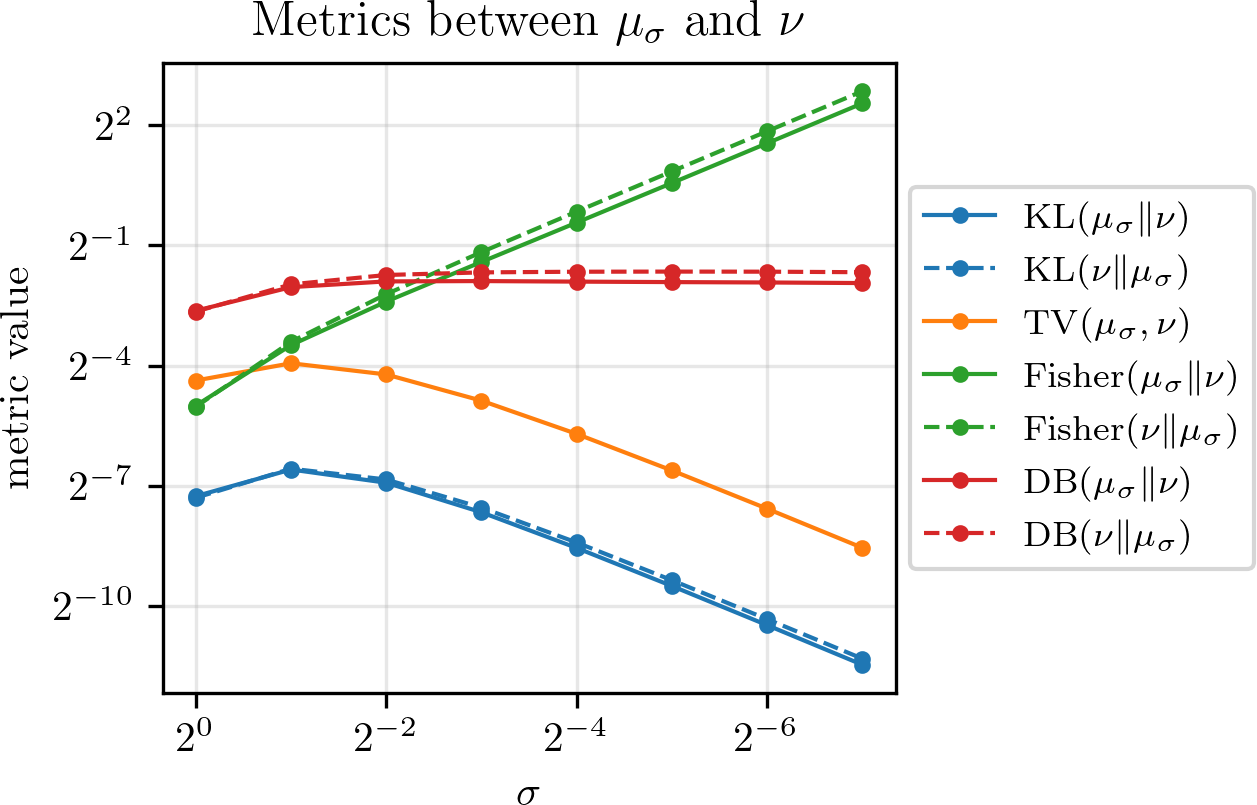
\includegraphics[width=0.6\linewidth]{../Codes/metric_compare/metrics.png}
    \caption{The four metrics between $\mu_\sigma$ and $\nu$ for $\sigma = 2^0, 2^{-1}, \dots, 2^{-7}$. KL and TV decay with $\sigma$; DB stays roughly constant; Fisher diverges.}
    \label{fig:metrics}
\end{figure}

\section{Single-step DB normalizing flow}\label{sec:single-step}

In this section we restrict attention to a single flow map $F$ trained in one shot to push the source onto the target; multi-step compositions are treated later. Let $U_0(x)$ and $U_1(x)$ be source and target potential functions on $\mathbb R^d$, and let $\mu_0(x) \propto \exp(-U_0(x))$ and $\mu_1(x) \propto \exp(-U_1(x))$ be the corresponding Boltzmann distributions. Given explicit samples from $\mu_0$, we aim to train a single flow map $F$ such that $F_{\#}\mu_0 = \mu_1$, with pushforward density
\begin{equation}\label{eq:pushforward}
    (F_{\#}\mu_0)(y) = \frac{\mu_0(x)}{|\det J_F(x)|}, \quad y = F(x),
\end{equation}
where $J_F(x) \in \mathbb R^{d\times d}$ is the Jacobian matrix of $F$. We start from the reverse-direction DB divergence $\DB(F_{\#}\mu_0\|\mu_1)$, since it integrates against the pushforward of the prior and can therefore be estimated entirely from $\mu_0$-samples that we have at hand, with no access to samples of $\mu_1$.

\subsection{Reverse DB loss and energy-based sampling}

First, we define the log importance weight
\begin{equation}\label{eq:WF-def}
    W_F(x) = \log \frac{(F_{\#}\mu_0)(F(x))}{\mu_1(F(x))} + \mathrm{const} = U_1(F(x)) - U_0(x) - \log|\det J_F(x)|.
\end{equation}
Viewing $W_F(x)$ as a function of $y = F(x)$, we have
\begin{equation*}
\nabla_y W_F(x) = \nabla \log (F_{\#}\mu_0)(y) - \nabla \log \mu_1(y).
\end{equation*}
Applying the DB divergence in~\eqref{eq:db-def} and the change of variable $y = F(x)$,
\begin{equation}\label{eq:db-reverse}
    \DB(F_{\#}\mu_0 \| \mu_1) = \int_{\mathbb R^d} (F_{\#}\mu_0)(y) |\nabla_y W_F(x)| \D y = \int_{\mathbb R^d} \mu_0(x) |\nabla_y W_F(x)| \D x.
\end{equation}

The gradient $\nabla_y W_F$ admits an explicit chain-rule expansion. Differentiating~\eqref{eq:WF-def} with respect to $y = F(x)$,
\begin{align}\label{eq:grad-W}
    \nabla_y W_F(x) & = \nabla U_1(F(x)) - \nabla_y\bigl(U_0(x) + \log|\det J_F(x)|\bigr) \notag\\
    & = \nabla U_1(F(x)) - J_F(x)^{-\top} \bigl(\nabla U_0(x) + \nabla \log|\det J_F(x)|\bigr).
\end{align}
Substituting~\eqref{eq:grad-W} into~\eqref{eq:db-reverse}, the loss in terms of the flow map $F$ takes the form
\begin{equation}\label{eq:loss-explicit}
    \DB(F_{\#}\mu_0 \| \mu_1) = \int_{\mathbb R^d} \mu_0(x) \Bigl|\nabla U_1(F(x)) - J_F(x)^{-\top} \bigl(\nabla U_0(x) + \nabla \log|\det J_F(x)|\bigr)\Bigr| \D x.
\end{equation}

The loss~\eqref{eq:loss-explicit} is highly nonlinear in $F$, primarily because of the explicit appearance of the Jacobian matrix $J_F(x)$ rather than only its determinant. Standard normalizing flow architectures such as RealNVP and NSF support efficient evaluation of the determinant, but assembling the full Jacobian costs at least $O(d^2)$, which becomes prohibitive in high dimensions even with automatic differentiation. The chain-rule form~\eqref{eq:grad-W} is therefore not a practical training target.

The way out is to estimate the gradient $\nabla_y W_F(x)$ stochastically along a random direction, never assembling $J_F(x)$ in full. Concretely, for $v \in \mathbb S^{d-1}$ we approximate the directional derivative $v^\top \nabla_y W_F(x)$ by central differences in $y = F(x)$. Fix a small step size $\varepsilon > 0$ and define
\begin{equation}\label{eq:xpm-reverse}
    x_{v\pm} = F^{-1}(F(x) \pm \varepsilon v),
\end{equation}
so that $F(x_{v\pm}) = F(x) \pm \varepsilon v$. Evaluating $W_F$ from~\eqref{eq:WF-def} at $x_{v\pm}$ and central-differencing in $y$ gives
\begin{equation}\label{eq:fd-reverse}
    v^\top \nabla_y W_F(x) \approx \frac{W_F(x_{v+}) - W_F(x_{v-})}{2\varepsilon},
\end{equation}
which by~\eqref{eq:WF-def} expands to
\begin{multline}\label{eq:fd-reverse-explicit}
    \frac{W_F(x_{v+}) - W_F(x_{v-})}{2\varepsilon} = \frac{U_1(F(x) + \varepsilon v) - U_1(F(x) - \varepsilon v)}{2\varepsilon} \\
    - \frac{\bigl(U_0(x_{v+}) + \log|\det J_F(x_{v+})|\bigr) - \bigl(U_0(x_{v-}) + \log|\det J_F(x_{v-})|\bigr)}{2\varepsilon}.
\end{multline}
The right-hand side requires only forward evaluations of $U_1$, $F^{-1}$, $U_0$, and $\log|\det J_F|$, all available cheaply in NSF-style architectures, and never assembles $J_F(x)$ itself. The reverse DB loss~\eqref{eq:db-reverse} is finally estimated by averaging $|v^\top \nabla_y W_F(x)|$ over $x \sim \mu_0$ and $v \sim \mathrm{Unif}(\mathbb S^{d-1})$:
\begin{equation}\label{eq:loss-reverse}
    \mathcal L_{\mathrm{reverse}}[F] = \mathbb E_{\substack{x \sim \mu_0 \\ v \sim \mathrm{Unif}(\mathbb S^{d-1})}} \biggl|\frac{W_F(x_{v+}) - W_F(x_{v-})}{2\varepsilon}\biggr|.
\end{equation}

\begin{remark}
The DB loss needs only $O(\sqrt d)$ random directions to recover the precision of a full-gradient evaluation, whereas a Fisher analogue needs $O(d)$, comparable to assembling $J_F(x)$ explicitly. To see this, recall that for $v \sim \mathrm{Unif}(\mathbb S^{d-1})$ and any $g \in \mathbb R^d$,
\begin{equation*}
    \mathbb E_v |v^\top g| = \frac{\Gamma(\frac{d}2)}{\sqrt{\pi}\, \Gamma(\frac{d+1}2)} |g| \sim \sqrt{\frac{2}{\pi d}} |g|, \qquad \mathbb E_v (v^\top g)^2 = \frac{1}{d} |g|^2,
\end{equation*}
where the asymptotic on the left follows from Stirling's formula. The DB integrand is $|g| = |\nabla_y W_F|$, scaling like $1/\sqrt d$, while the Fisher integrand is $|g|^2$, scaling like $1/d$. The directional-derivative trick is therefore well matched to the DB normalizing flow but offers no asymptotic saving for its Fisher analogue.
\end{remark}

\subsection{Forward DB loss and mode guiding}

Similar to the reverse DB loss, the forward DB loss $\DB(\mu_1\|F_{\#}\mu_0)$ can be written as
\begin{equation}\label{eq:db-forward}
    \DB(\mu_1\|F_{\#}\mu_0) = \int_{\mathbb R^d} \mu_1(y) |\nabla_y W_F(x)| \D y,
\end{equation}
the only difference from~\eqref{eq:db-reverse} being that the integration measure is the target $\mu_1$ rather than the prior $\mu_0$. The same central-difference scheme as in~\eqref{eq:fd-reverse} applies: for a fixed $y \in \mathbb R^d$, set
\begin{equation}\label{eq:xpm-forward}
    x_{v\pm} = F^{-1}(y \pm \varepsilon v),
\end{equation}
so that $F(x_{v\pm}) = y \pm \varepsilon v$, and approximate $v^\top \nabla_y W_F(x)$ at $x = F^{-1}(y)$ by
\begin{multline}\label{eq:fd-forward-explicit}
    \frac{W_F(x_{v+}) - W_F(x_{v-})}{2\varepsilon} = \frac{U_1(y + \varepsilon v) - U_1(y - \varepsilon v)}{2\varepsilon} \\
    - \frac{\bigl(U_0(x_{v+}) + \log|\det J_F(x_{v+})|\bigr) - \bigl(U_0(x_{v-}) + \log|\det J_F(x_{v-})|\bigr)}{2\varepsilon},
\end{multline}
yielding the forward loss
\begin{equation}\label{eq:loss-forward}
    \mathcal L_{\mathrm{forward}}[F] = \mathbb E_{\substack{y \sim \mu_1 \\ v \sim \mathrm{Unif}(\mathbb S^{d-1})}} \biggl|\frac{W_F(x_{v+}) - W_F(x_{v-})}{2\varepsilon}\biggr|.
\end{equation}
The only difference from~\eqref{eq:loss-reverse} is that $y$ is drawn from the target $\mu_1$, so the computation graph tracks $y$ rather than $x = F^{-1}(y)$.

\begin{remark}
    Unlike the KL divergence, which is invariant under pushforward by a diffeomorphism, the DB divergence is not; in general
    \begin{equation*}
        \DB(\mu_1\|F_{\#}\mu_0) \neq \DB(F^{-1}_{\#}\mu_1\|\mu_0),
    \end{equation*}
    because a change of variable transforms the score difference by the Jacobian factor $J_F^\top$, whose $L^1$ norm is not preserved unless $F$ is an isometry. In principle, $\DB(F^{-1}_{\#}\mu_1\|\mu_0)$ could also serve as a forward DB loss, but we keep $\DB(\mu_1\|F_{\#}\mu_0)$ because its derivation is simpler.
\end{remark}

The forward loss $\mathcal L_{\mathrm{forward}}[F]$ in~\eqref{eq:loss-forward} cannot be evaluated directly, since it requires explicit samples from the target $\mu_1$, which is exactly what the Boltzmann generator is supposed to produce. We circumvent this by exploiting a structural property of the DB divergence that has no analogue in KL.

\emph{Key principle.} Because the DB integrand $|\nabla_y W_F(x)|$ is pointwise nonnegative, replacing $\mu_1$ in~\eqref{eq:loss-forward} by any positive measure $\hat\mu_1$ yields a surrogate loss $\hat{\mathcal L}_{\mathrm{forward}}[F]$ that still vanishes exactly when $F_{\#}\mu_0 \propto \mu_1$ on $\mathrm{supp}(\hat\mu_1)$, so the global minimizer is preserved regardless of how $\hat\mu_1$ is chosen. KL has no such freedom: its integrand $\log(\mu_1/F_{\#}\mu_0)$ is signed, so any inaccuracy in $\mu_1$ shifts the optimum to $F_{\#}\mu_0 = \hat\mu_1$, and KL training therefore demands exact samples from $\mu_1$. For DB it suffices that $\mathrm{supp}(\hat\mu_1)$ covers the modes the reverse loss tends to drop, freeing us to choose any tractable guiding measure.

A Gaussian mixture is a convenient choice since it can be sampled directly:
\begin{equation}\label{eq:hat-mu1}
    \hat\mu_1(y) = \sum_{i=1}^n w_i\, \mathcal N(y; x_i, \Sigma_i), \qquad w_i \Ge 0.
\end{equation}
Linearity then expands $\hat{\mathcal L}_{\mathrm{forward}}[F]$ as a per-component sum,
\begin{equation}\label{eq:hat-loss-forward}
    \hat{\mathcal L}_{\mathrm{forward}}[F] = \sum_{i=1}^n w_i\, \mathbb E_{\substack{y \sim \mathcal N(x_i, \Sigma_i) \\ v \sim \mathrm{Unif}(\mathbb S^{d-1})}} \biggl|\frac{W_F(x_{v+}) - W_F(x_{v-})}{2\varepsilon}\biggr|,
\end{equation}
with $x_{v\pm}$ as in~\eqref{eq:xpm-forward}. The total loss is then simply
\begin{equation}\label{eq:total-loss}
    \mathcal L_{\mathrm{total}}[F] = \mathcal L_{\mathrm{reverse}}[F] + \hat{\mathcal L}_{\mathrm{forward}}[F].
\end{equation}
The guidance term supplies mode information from the target side and effectively suppresses the mode collapse that pure energy-based normalizing flows commonly suffer from.

\begin{remark}
    Mode guidance has also been considered in Jeffreys Flow~\citep{lin2026jeffreys}, but the construction there is based on the KL divergence and therefore requires accurate samples from the target $\mu_1$ to remain unbiased. The DB-based guidance proposed here is unbiased for any choice of $\hat\mu_1$ whose support covers the target modes, which is the property that the signed KL integrand cannot provide.
\end{remark}

For notational convenience, we denote the flow map produced by the DB normalizing flow training as
\begin{equation}
    F = \mathrm{DBNF}\bigl(U_0, \mu_0;\, U_1, \hat\mu_1\bigr),
\end{equation}
indicating that $F$ minimizes the DB divergence built from the potentials $U_0, U_1$, with $\mu_0$ providing the source samples and the guiding measure $\hat\mu_1$ providing the auxiliary mode guidance.

\subsection{Choice of guiding measure}

Although the DB normalizing flow allows the guiding measure $\hat\mu_1$ to be chosen flexibly without disturbing the global minimizer, the actual choice of $\hat\mu_1$ is delicate in practice. In the simplest case, when $\mu_0$ and $\mu_1$ are far from each other, one can simulate Langevin dynamics or run SMC to obtain approximate samples from $\mu_1$ and use them as the guiding measure. However, such methods still rely essentially on ergodicity, and may encounter difficulty when the target distribution is concentrated on a low-dimensional manifold.

We propose instead a curvature-targeted construction that directly addresses this failure mode: rather than waiting for an ergodic sampler to discover sharp basins of $U_1$, we identify them analytically from the potential and place mixture centers there. Define the mode weight function
\begin{equation}
    M(x) := \frac{|\nabla^2 U_1(x)|}{|\nabla U_1(x)|+\delta},
\end{equation}
where $\delta>0$ regularizes the denominator to avoid singularity. The ratio is large precisely where $U_1$ has small gradient and large curvature, i.e.\ near a local minimum with a sharp basin, which are exactly the modes the reverse loss is most prone to drop. We apply $M(x)$ as a reweighting to the source distribution $\mu_0(x)$ and resample from $M(x) \mu_0(x)$, using the resulting points as centers of the guiding measure.

Computing $\nabla^2 U_1(x)$ exactly from a gradient oracle alone is unnecessarily expensive; instead we use a kernel-smoothed surrogate that needs only gradient evaluations,
\begin{equation}
    |\nabla^2 U_1(x)| \approx H(x) := \frac{\displaystyle \int_{\mathbb R^d} \max\biggl[\frac{|\nabla U_1(x) - \nabla U_1(y)|}{|x-y|}, A\biggr] e^{-\frac{|x-y|^2}{2\sigma^2}} \mu_0(y) \D y}{\displaystyle \int_{\mathbb R^d} e^{-\frac{|x-y|^2}{2\sigma^2}} \mu_0(y) \D y},
\end{equation}
which introduces an additional parameter $\sigma>0$. In practice, we choose the parameters as
\begin{subequations}\label{eq:dsa-params}
\begin{align}
    \delta &= 0.01 \int_{\mathbb R^d} |\nabla U_1(x)| \mu_0(x) \D x, \label{eq:param-delta}\\
    \sigma &= 0.1 \int_{\mathbb R^{2d}} |x-y| \mu_0(x) \mu_0(y) \D x \D y, \label{eq:param-sigma}\\
    A &= \int_{\mathbb R^{2d}} \frac{|\nabla U_1(x) - \nabla U_1(y)|}{|x-y|} \mu_0(x) \mu_0(y) \D x \D y. \label{eq:param-A}
\end{align}
\end{subequations}

Suppose we resample $x_1,\dots,x_n$ from the weighted distribution $M(x) \mu_0(x)$. Then we define the Gaussian mixture guiding measure
\begin{equation}
    \hat\mu_1(y) = \frac{\lambda}n \sum_{i=1}^n \mathcal N\bigl(y;x_i,H^{-1}(x_i)\bigr).
\end{equation}
The centers $x_i$ are concentrated in regions of high mode weight, and the covariance $H^{-1}(x_i)$ scales each component to the local basin width, so sharp basins receive narrow Gaussians and broad basins receive wide ones, which is the natural choice once $H$ is interpreted as a curvature surrogate. The scalar $\lambda > 0$ is a user-chosen parameter that tunes the overall strength of the mode guidance relative to the reverse loss; since $\hat\mu_1$ enters the DB loss only as a positive measure, $\lambda$ does not need to normalize $\hat\mu_1$ to a probability density.

The full procedure for a single DB flow step is summarized in Algorithm~\ref{alg:dbnf-step}.

\begin{algorithm}[h]
    \setstretch{1.2}
    \DontPrintSemicolon
    \caption{Single DB normalizing flow step}\label{alg:dbnf-step}
    \KwIn{source potential $U_0$ with samples from $\mu_0$; target potential $U_1$; guidance strength $\lambda > 0$.}
    \KwOut{flow map $F$ with $F_{\#}\mu_0 \approx \mu_1$.}
    Estimate the parameters $\delta$, $\sigma$, $A$ in~\eqref{eq:dsa-params} by Monte Carlo over $\mu_0$ samples.\;
    Evaluate the curvature surrogate at each $\mu_0$ sample,
    \begin{equation*}
        H(x) = \frac{\displaystyle \int_{\mathbb R^d} \max\biggl[\frac{|\nabla U_1(x) - \nabla U_1(y)|}{|x-y|}, A\biggr] e^{-\frac{|x-y|^2}{2\sigma^2}} \mu_0(y) \D y}{\displaystyle \int_{\mathbb R^d} e^{-\frac{|x-y|^2}{2\sigma^2}} \mu_0(y) \D y}.
    \end{equation*}

    Evaluate the mode weight at each $\mu_0$ sample,
    \begin{equation*}
        M(x) = \frac{H(x)}{|\nabla U_1(x)| + \delta}.
    \end{equation*}

    Resample $x_1,\dots,x_n$ from the reweighted distribution $M(x)\mu_0(x)$.\;
    Form the guiding measure
    \begin{equation*}
        \hat\mu_1(y) = \frac{\lambda}n \sum_{i=1}^n \mathcal N\bigl(y; x_i, H^{-1}(x_i)\bigr).
    \end{equation*}

    Train $F = \mathrm{DBNF}(U_0,\mu_0;\, U_1,\hat\mu_1)$ by minimizing $\mathcal L_{\mathrm{total}}[F]$ in~\eqref{eq:total-loss}.\;
\end{algorithm}

\section{DB Boltzmann generator}\label{sec:db-bg}

\bibliographystyle{plainnat}
\bibliography{references}

\end{document}